\documentclass[a4paper, 11pt, twocolumn]{IEEEtran}

\usepackage{graphicx}
\usepackage[scale=.8]{geometry}
\usepackage{microtype}

\title{Some title for a multimodal chess interface}
\author{Giuseppina Iannotti, and Davide Marincione}
\date{11th of June, 2024}

\begin{document}
    \maketitle
    \begin{abstract}
        This is the abstract.
    \end{abstract}

    \section{Introduction}

    {\Huge This intro has to change!}\\
    In this report, we present the design, implementation, and testing, of a multimodal interface for playing chess. The interface allows the user to play with either mouse movements, hand gestures or voice commands. The user can switch between the different modalities at any time during the game. It is implemented in \texttt{python} and uses the \texttt{pygame} library for the audio-visual inteface, \texttt{opencv} and \texttt{mediapipe} for hand gesture recognition, and the \texttt{dragonfly} library for voice commands. The interface has been tested with a group of 12 users, and the results show that the multimodal interface is more engaging and fun to use than a traditional mouse-based interface.

    \section{Coding, Graphics \& Audio}
    \paragraph*{Libraries} A chess program is quite complex to make, and since writing one would've been a project in itself, we have decided to use the \texttt{python-chess} library. This choice enabled us to abstract away the complexity of the game, and to focus on making the interface and the interaction. \texttt{python-chess} is used all over the project's code, to make checks and queries to display the correct information, but also to interact with the chess engine and to make moves.\\For the graphics, audio and event handling, we used the \texttt{pygame} library, which is a set of \texttt{python} modules designed for writing small video games. It is simple yet very powerful, as it allows to draw shapes, images and text on the screen, to play sounds, and to handle user input. Admittedly, it can be quite slow for medium to large-scale projects, as its main drawback is the graphics rendering, which is done via old-fashioned blitting. But, for a project such as ours, it was more than enough.

    \paragraph*{Programming paradigm} For all its usefullness, \texttt{pygame} only provides basic functionalities and none of the data structures and systems used in writing videogames. Things that, to a certain extent, we needed for our project. So we decided to go for an OOP approach, defining ever more refined objects, building on top of more abstract ones. This tactic proved to be extremely successful, as in the later parts of the project there were a couple of instances in which we needed a new class, and we were able to define it without much hassle.
    \begin{figure*}\label{fig:uml}
        \centering
        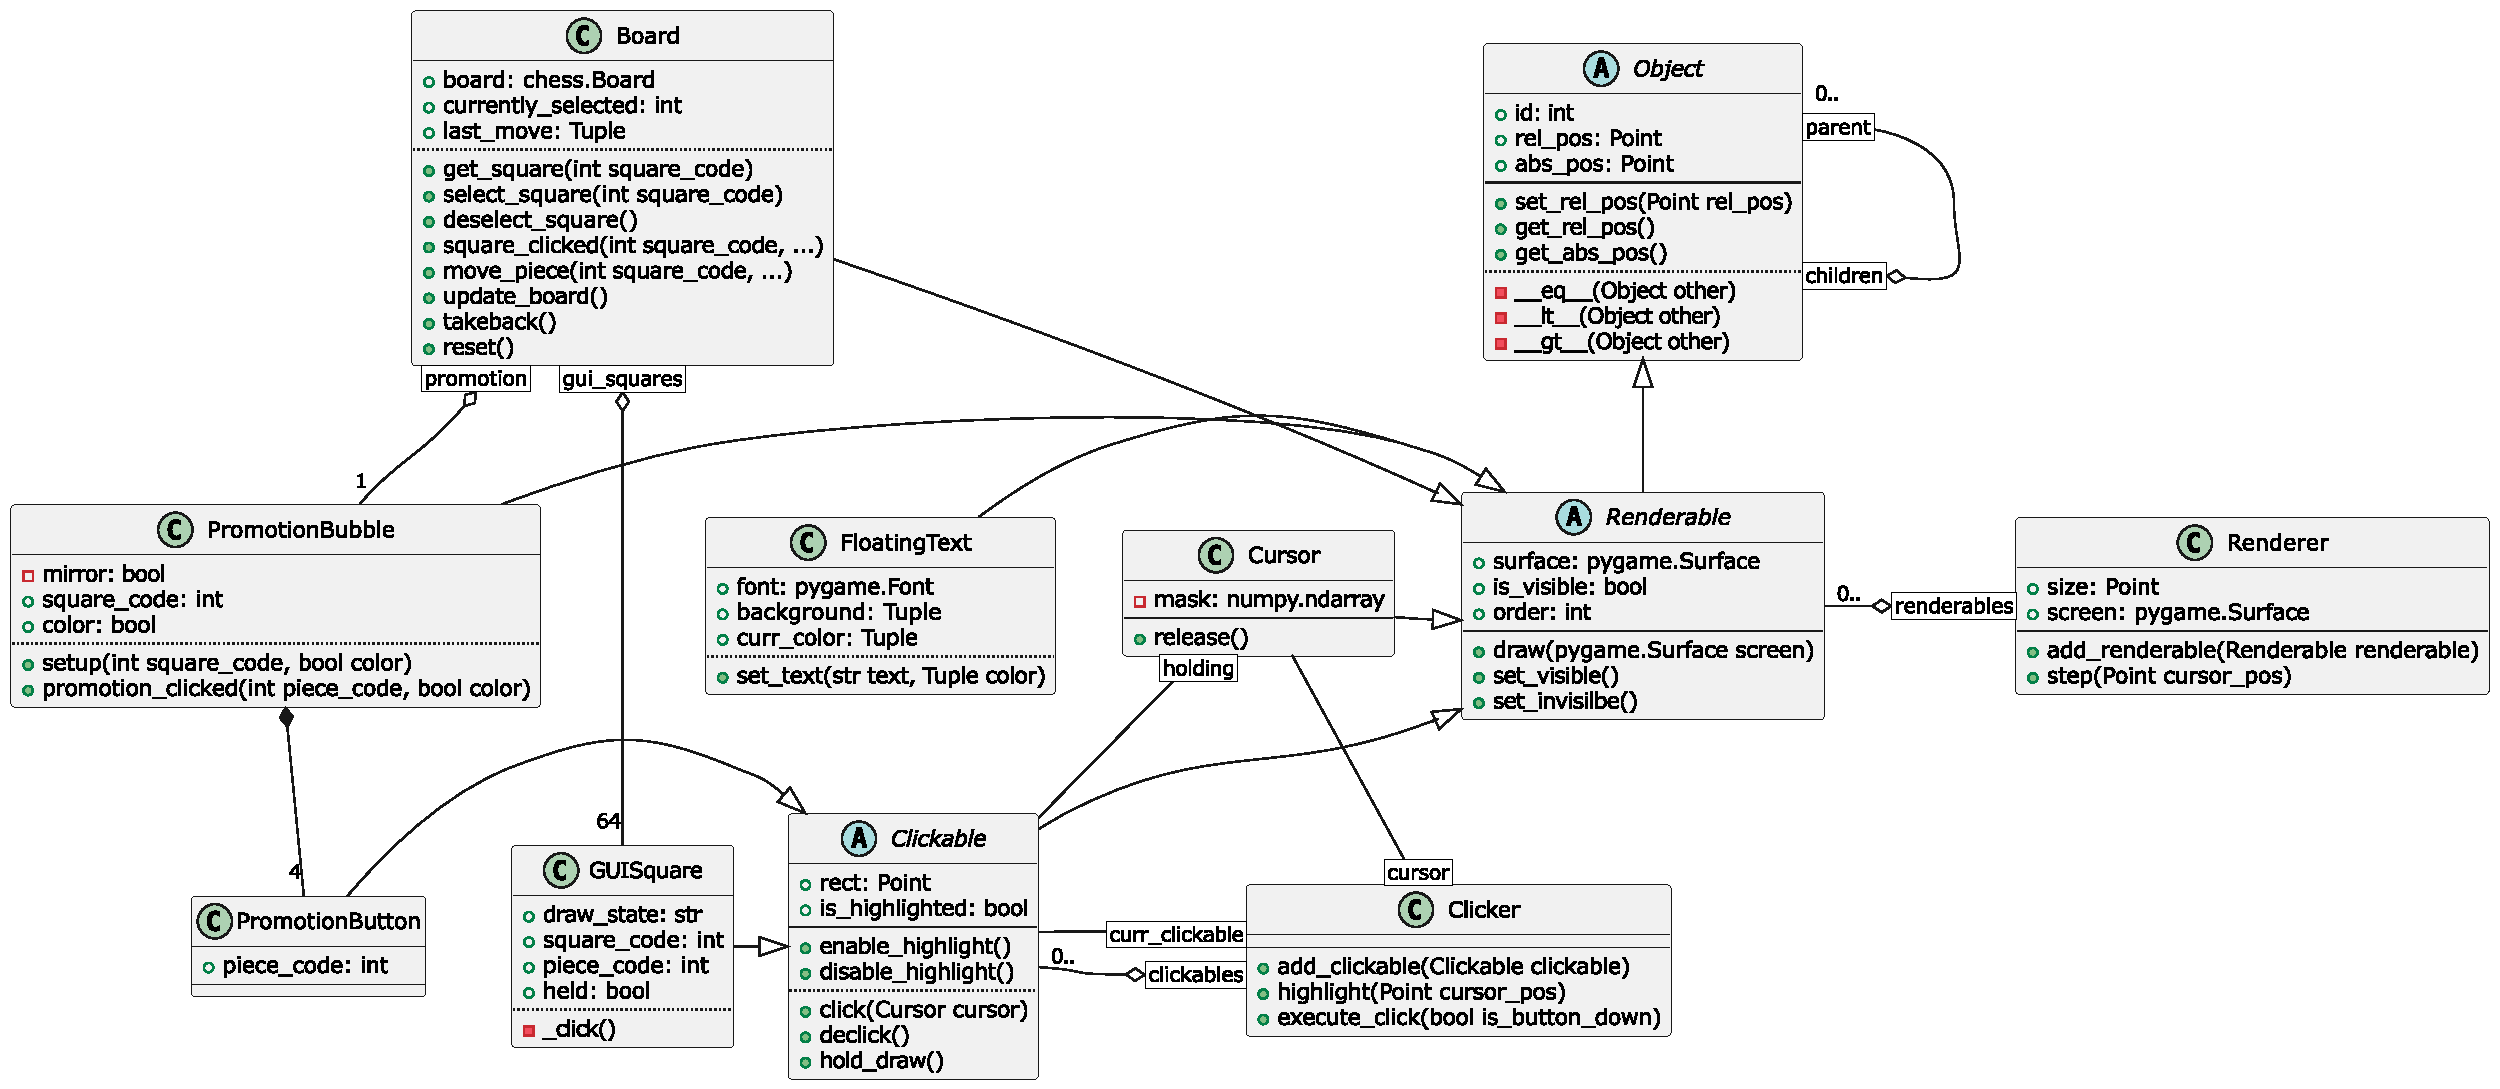
\includegraphics[width=.8\textwidth]{uml.pdf}
        \caption{UML description of the basic structure of the program.}
    \end{figure*}
    \paragraph*{Basic structure} Inspired by many game engines (Unity, Godot, etc.), our first class was the \texttt{Object} class, which is the base class for all the elements in our program. It is defined to be as generic as possible: an object in 2d space which, being in a parent-child hierarchy, can have its absolute position changed by the parent, while maintaining its relative position to it.

    \section{Hand gestures}

    \section{Voice commands}

    \section{Experiments and Results}

    \section{Conclusions}

\end{document}
